\documentclass[a4paper,12pt]{article}
\usepackage[margin=1in]{geometry}
\usepackage{fancyhdr}
%\usepackage{graphicx}
\pagestyle{fancy}

\usepackage{amsmath}
\usepackage{amsthm}
\usepackage{amssymb}
\usepackage{mathtools}
%\usepackage{algorithm2e}
\usepackage{listings}

%To display code
\usepackage{minted}
\usepackage{xcolor} % to access the named colour LightGray
\definecolor{LightGray}{gray}{0.9}
%\rmand{\MintedPygmentize}{~/usr/bin/pygmentize}


%%% CAPTIONS
\usepackage{caption}
\usepackage{subcaption}
\DeclareCaptionFormat{custom}
{%
    \textbf{#1#2}\textit{\small #3}
}
\captionsetup{format=custom}



\newtheorem{theorem}{Theorem}[section]
\newtheorem{lemma}[theorem]{Lemma}
\newtheorem*{theorem*}{Theorem}

\usepackage{tikz}
    \usetikzlibrary{shapes,arrows}
    \usetikzlibrary{arrows,calc,positioning}

    \tikzset{
        block/.style = {draw, rectangle,
            minimum height=1cm,
            minimum width=1.5cm},
        input/.style = {coordinate,node distance=1cm},
        output/.style = {coordinate,node distance=4cm},
        arrow/.style={draw, -latex,node distance=2cm},
        pinstyle/.style = {pin edge={latex-, black,node distance=2cm}},
        sum/.style = {draw, circle, node distance=1cm},
    }

\usepackage{dirtytalk}
\usepackage{floatrow}
\usepackage{mwe}

\usepackage{xcolor}
\usepackage{lipsum}
\usepackage{geometry} % Required for adjusting page dimensions and margins
\usepackage[framemethod=tikz]{mdframed}
\makeatletter
\let\ps@plain\ps@fancy
  \ifcsname f@nch@setoffs\endcsname\else%
  \let\f@nch@setoffs\fancy@setoffs
\fi
\makeatother
\pagestyle{fancy}
\renewcommand{\headrulewidth}{0.4pt}\renewcommand{\footrulewidth}{0.4pt}
\lhead{Hi}\rhead{Bye}
\makeatletter
\newcommand{\resetHeadWidth}{\f@nch@setoffs}
\makeatother


%----------------------------------------------------------------------------------------
%	DOCUMENT MARGINS
%----------------------------------------------------------------------------------------


\geometry{
	paper=a4paper, % Paper size, change to letterpaper for US letter size
	top=2.5cm, % Top margin
	bottom=1.5cm, % Bottom margin
	left=1.5cm, % Left margin
	right=1.5cm, % Right margin
	headheight=40pt, % Header height
	footskip=0.5cm, % Space from the bottom margin to the baseline of the footer
	headsep=0.5cm, % Space from the top margin to the baseline of the header
	%showframe, % Uncomment to show how the type block is set on the page
}
\resetHeadWidth
\pagestyle{fancy}
\fancyhf{}
\rfoot{Page \thepage \hspace{1pt}}
\lhead{LA Project}
\rhead{
\includegraphics[width=3cm]{iiit-new.png}}
%-----------------------------------------------------------------------------


%Borrowed-----------------------------------------------------------------------------
%\usepackage{lgrind}        % convert program listings to a form includable in a LaTeX document
\usepackage{chapterbib}    % allows a bibliography for each chapter (each labguide has it's own)
\usepackage{color}         % produces boxes or entire pages with colored backgrounds
\usepackage{graphics}      % standard graphics specifications
%\usepackage[pdftex]{graphicx}      % alternative graphics specifications
\usepackage{longtable}     % helps with long table options
\usepackage{epsf}          % old package handles encapsulated post script issues
\usepackage{bm}            % special 'bold-math' package
\usepackage{verbatim}			% for comment environment
%\usepackage{asymptote}     % For typesetting of mathematical illustrations
%\usepackage{thumbpdf}
\usepackage[colorlinks=true]{hyperref}  % this package should be added after all others
%-----------------------------------------------------------------------------

%----------------------------------------------------------------------------------------
%	NUMBERED QUESTIONS ENVIRONMENT
%----------------------------------------------------------------------------------------

\newenvironment{problem}[2][Problem]
    { \begin{mdframed}[backgroundcolor=gray!20] \textbf{#1 #2} \\}
    {  \end{mdframed}}

% Define solution environment
\newenvironment{solution}
    {\textit{Solution:}}
    {}


% Usage:
% \begin{question}[optional title]
%	Question contents
% \end{question}

\mdfdefinestyle{question}{
	innertopmargin=1.2\baselineskip,
	innerbottommargin=0.8\baselineskip,
	roundcorner=5pt,
	nobreak,
	singleextra={%
		\draw(P-|O)node[xshift=1em,anchor=west,fill=white,draw,rounded corners=5pt]{%
		Question \theQuestion\questionTitle};
	},
}

\newcounter{Question} % Stores the current question number that gets iterated with each new question

% Define a custom environment for numbered questions
\newenvironment{question}[1][\unskip]{
	\bigskip
	\stepcounter{Question}
	\newcommand{\questionTitle}{~#1}
	\begin{mdframed}[style=question]
}{
	\end{mdframed}
	\medskip
}

\newtheorem{Theorem}{Theorem}[section]
\newtheorem{Proposition}[Theorem]{Proposition}
\newtheorem{Lemma}[Theorem]{Lemma}
\newtheorem{Definition}[Theorem]{Definition}
\newtheorem{Corollary}[Theorem]{Corollary}
\newtheorem{Remark}[Theorem]{Remark}

\begin{document}
%----------------------------------------------------------------------------------------
%	DOCUMENT TITLE
%----------------------------------------------------------------------------------------

\title{MA2.101: Linear Algebra - Project \\ \textbf{\textit{Unraveling Genetic Patterns with Linear Algebra}}} % Title of the assignment

\author{Chetan Mahipal\\ \\ Course Instructor - Dr. Chittaranjan Hens} % Author name and email address
\date{IIIT Hyderabad - \today} % University, school and/or department name(s) and a date1
\maketitle
\textit{\say{Genetics is the key to our past, present, and future, and linear algebra provides us with the language to decode its secrets.}} - Anonymous.
\begin{abstract} 
\ \\
Genetics research has witnessed an explosion of data in recent years, requiring advanced analytical approaches to extract meaningful insights. This project explores the integration of linear algebra and genetics to uncover underlying patterns and structures within genetic data. By leveraging matrix operations, eigenvalue analysis, and dimensionality reduction techniques, we aim to gain a comprehensive understanding of gene interactions, disease susceptibility, and evolutionary processes. Through the application of linear algebraic tools to gene expression profiles, genetic networks, and population genetics, we reveal hidden relationships, identify key genetic factors, and shed light on the mechanisms underlying complex biological systems. This project underscores the significance of linear algebra as a powerful tool for analyzing genetic data and provides a foundation for future investigations in the field of genetics research.

% the agents of a number of diseases characterized by slow progressive neurological degeneration which was fatal.
\end{abstract}
 % Print the title
\section{Introduction}
\subsection{Alleles and Genotypes}

In genetics, an allele refers to one of the alternative forms of a gene that occupies a specific position, or locus, on a chromosome. Alleles are responsible for the variations observed in inherited traits among individuals. For example, in the context of eye color, there can be alleles for blue eyes, brown eyes, and so on.

A genotype, on the other hand, refers to the combination of alleles that an individual possesses for a particular gene or set of genes. It represents the genetic makeup of an organism. Genotypes can be represented by letters, with uppercase letters typically used to represent dominant alleles and lowercase letters for recessive alleles. For instance, in the case of eye color, a genotype might be represented as BB for someone with two alleles for brown eyes or Bb for someone with one allele for brown eyes and one allele for blue eyes.

The study of alleles and genotypes is essential in understanding inheritance patterns, genetic diversity, and the transmission of traits across generations. By analyzing allele frequencies and genotypic ratios, geneticists can gain insights into the inheritance of specific traits and how they may be influenced by various factors such as natural selection or genetic drift. \ \\
\begin{figure}[h]
\centering
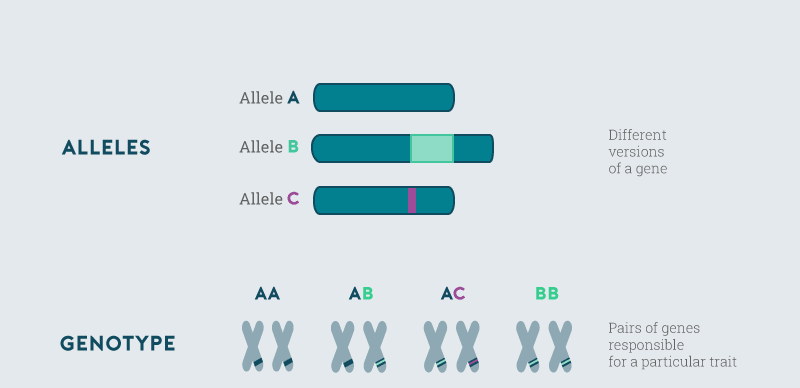
\includegraphics[width=0.6\textwidth]{Alleles.png}
\caption{Formation of Genotypes from Alleles.}
\label{fig:Punett-table}
\end{figure}
\subsection{Brief about Autosomal Inheritance}
According to Cubero (2013), autosomal inheritance involves the transmission of genetic traits or conditions from parents to offspring. Individuals inherit one gene from each parent, forming their own pair of genes. The specific gene passed on to an offspring is determined by chance. In the context of classifying individuals in a population based on their genotypes, three types of genotypes can be observed: AA, Aa, and aa. It is worth noting that the genotype Aa is the same as aA.

By classifying individuals into these genotypic categories, it becomes possible to determine the proportions of each genotype within a population. This information is essential for understanding the distribution and prevalence of specific alleles within a population. It allows researchers to gain insights into the genetic composition of a population and study how traits or conditions are inherited across generations.
\section{Foundational Concepts and Terminology}
\subsection{Proportions of Alleles in a Population}
To determine the proportions of alleles in the population, we can consider the proportions of each genotype in different generations. Let's denote these proportions for the generation of order n as p\textsubscript{n} for AA, q\textsubscript{n} for Aa, and r\textsubscript{n} for aa.

For n = 0, 1, 2, ..., the following relationships hold:\ \\
p\textsubscript{n} represents the proportion of the AA genotype in the generation of order n.\ \\
q\textsubscript{n} represents the proportion of the Aa genotype in the generation of order n.\ \\
r\textsubscript{n} represents the proportion of the aa genotype in the generation of order n.\ \\

Assuming that these proportions can be determined, note that one must have the equality, u = p\textsubscript{n} + q\textsubscript{n} + r\textsubscript{n} Then, the proportions u and v of the two alleles A and a in the population satisfy the following equations.

\begin{enumerate}
\item \( u = p_{n} + \frac{1}{2}q_{n} \)
\item \( v = \frac{1}{2}q_{n} + r_{n} \)
\end{enumerate}
Here, we used the fact that the A and a alleles constitute 100\% of the AA genotype (with proportion p\textsubscript{n}) and 50\% each of the Aa genotype. Similarly, for the alleles, if it is assumed that the genotypes occur in the same proportions between males and females, then u and v represent (in the entire population) the probabilities that the gene is A or a, respectively
\subsection{Punett Tables}
\subsubsection{Introduction}
In the field of genetics, a powerful tool called the Punnett square is used to visualize and predict the possible combinations of genes that can occur when two organisms with known genotypes are crossed. This technique is named after the renowned English geneticist Reginald Punnett, who made significant contributions to the field of genetics, including his work on sex linkage and sex determination. Punnett's research also involved studying feather color characteristics in chickens, both in male and female individuals.
\subsubsection{Construction of Punett Squares}
A Punnett square is constructed by organizing the possible alleles from each parent along the axes of a square grid. The alleles are represented by letters, such as A and a, to denote different genetic variants. The combinations in the square represent the potential genotypes of the offspring resulting from the cross.\ \\
To illustrate how a Punnett square is constructed, it should be noted that if one parent is of the Aa genotype, then it is equally likely that the offspring will inherit either the A allele or a allele from this parent. On the other hand, if one parent is of genotype aa and the other is of genotype Aa, the offspring will always receive a allele from the genotype aa parent and an A or a allele, with equal probability, from the genotype Aa parent. Thus, the offspring has the same probability of being of genotype AA or Aa.
\begin{figure}[h]
\centering
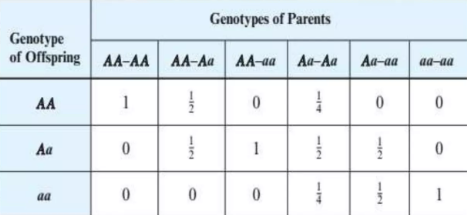
\includegraphics[width=0.6\textwidth]{Di_Hybrid_Cross.png}
\caption{Probabilities of the possible genotypes of the offspring for all possible combinations of the genotypes of the parents.}
\label{fig:Punett-table}
\end{figure}
\subsection{Hardy-Weinberg Law}
The Hardy-Weinberg law, also known as the Hardy-Weinberg equilibrium, is a fundamental principle in population genetics that describes the relationship between the frequencies of alleles and genotypes in a population under certain assumptions.

The law is based on the following key assumptions:
\begin{enumerate}
  \item Random Mating: Individuals in the population mate randomly with respect to the gene in question.
  \item No Mutations: There are no new mutations occurring in the gene.
  \item No Migration: There is no migration of individuals into or out of the population.
  \item No Natural Selection: There is no differential survival or reproduction based on the genotype.
  \item Large Population Size: The population is infinitely large, or at least large enough to prevent random fluctuations in allele frequencies (genetic drift).
\end{enumerate}

Under these assumptions, the Hardy-Weinberg law predicts that the frequencies of alleles and genotypes in a population will remain constant from generation to generation. The law states that in the absence of evolutionary forces, such as selection or genetic drift, the genotype frequencies stabilize and reach an equilibrium state. This equilibrium can be calculated based on the initial genotype frequencies and the allele frequencies in the population.
\section{Case Study- Genotype Distribution in a Cropping Program}
\subsection{Problem Statement}
A farmer is managing a large population of plants with three possible genotypes: AA, Aa, and aa. The farmer aims to implement a cropping program wherein all plants in the population are fertilized by a plant of genotype AA. The objective is to determine the formula for the distribution of the three possible genotypes in the population after a certain number of generations.
\subsection{Solution}
To determine the long-term distribution of genotypes in the population, we use the matrix notation derived from the equations defining the distribution in each generation. Let $\mathbf{X}(n) = [p\ q\ r]$ represent the proportions of the three genotypes (AA, Aa, and aa) in the generation of order $n$. The equations can be expressed in matrix form as:

\[
\mathbf{X}^{(n)} = P\mathbf{X}^{(n-1)}, \quad \text{for } n = 0, 1, 2, \ldots, \tag{1}
\]

\[
X^{(n)} = \begin{bmatrix} p_{n} \\ q_{n} \\ r_{n}\end{bmatrix}, \quad X^{(n-1)} = \begin{bmatrix} p_{n-1} \\ q_{n-1} \\ r_{n-1} \end{bmatrix}
\]


where $P$ is the transition matrix. The matrix $\mathbf{X}^{(0)}$ represents the initial proportions of genotypes in the population.

We have $P = \begin{bmatrix} 1 & \frac{1}{2} & 0 \\ 0 & \frac{1}{2} & 1 \\ 0 & 0 & 0 \end{bmatrix}$ as the transition matrix, which corresponds to the given Punnett square probabilities.
From Equation (1), it follows that
\[
\mathbf{X}^{(n)} = P\mathbf{X}^{(n-1)} =P^{2}\mathbf{X}^{(n-2)}=\ldots=P^{n}\mathbf{X}^{(0)} \tag{2}
\]

The eigenvalues of $P$ can be found by solving the characteristic equation:

\[
\text{det}(P - \lambda I) = 0,
\]
where $\lambda$ is the eigenvalue and $I$ is the identity matrix. Solving this equation gives us three eigenvalues: $\lambda_1 = 1$, $\lambda_2 = \frac{1}{2}$, and $\lambda_3 = 0$.
\
To find the corresponding eigenvectors, we substitute each eigenvalue into the equation $(P - \lambda I)\mathbf{v} = \mathbf{0}$, where $\mathbf{v}$ is the eigenvector. 
\newpage
\ \\
Solving these equations yields the following eigenvectors: $\mathbf{v}_1 = \begin{bmatrix} 1 \\ 0 \\ 0 \end{bmatrix}$, $\mathbf{v}_2 = \begin{bmatrix} 1 \\ -1 \\ 0 \end{bmatrix}$, and $\mathbf{v}_3 = \begin{bmatrix} \frac{1}{2} \\ -1 \\ \frac{1}{2} \end{bmatrix}$.
Using these eigenvalues and eigenvectors, we can express $P$ as a diagonalizable matrix $CDC^{-1}$, where $D$ is the diagonal matrix containing the eigenvalues and $C$ is the matrix with the eigenvectors as columns.


\begin{align*}
C &= \begin{bmatrix} 1 & 1 & \frac{1}{2} \\ 0 & -1 & -1 \\ 0 & 0 & \frac{1}{2} \end{bmatrix}, \\
D &= \begin{bmatrix} \lambda_1 & 0 & 0 \\ 0 & \lambda_2 & 0 \\ 0 & 0 & \lambda_3 \end{bmatrix} = \begin{bmatrix} 1 & 0 & 0 \\ 0 & \frac{1}{2} & 0 \\ 0 & 0 & 0 \end{bmatrix}
\end{align*}

\ \\
Now, as we have already determined the matrices $C$ and $D$, we can find the value of $P^{(n)}$ as $P^{(n)} = CD^nC^{-1}$.

\[
P^{(n)} = \begin{bmatrix} 1 & 1 & \frac{1}{2} \\ 0 & -1 & -1 \\ 0 & 0 & \frac{1}{2} \end{bmatrix} \begin{bmatrix} 1^n & 0 & 0 \\ 0 & \left(\frac{1}{2}\right)^n & 0 \\ 0 & 0 & 0^n \end{bmatrix} \begin{bmatrix} 1 & 1 & \frac{1}{2} \\ 0 & -1 & -1 \\ 0 & 0 & \frac{1}{2} \end{bmatrix}^{-1} 
\]
From Equation (2), it follows that
$X^{(n)} = CD^nC^{-1}X^{(0)}$\\
\begin{align}
\implies 
X^{(n)} &= \begin{bmatrix} 1 & 1 & \frac{1}{2} \\ 0 & -1 & -1 \\ 0 & 0 & \frac{1}{2} \end{bmatrix} \begin{bmatrix} 1^n & 0 & 0 \\ 0 & \left(\frac{1}{2}\right)^n & 0 \\ 0 & 0 & 0^n \end{bmatrix} \begin{bmatrix} 1 & 1 & \frac{1}{2} \\ 0 & -1 & -1 \\ 0 & 0 & \frac{1}{2} \end{bmatrix}^{-1} \begin{bmatrix} p_{0} \\ q_{0} \\ r_{0}\end{bmatrix}\nonumber\\
&=\begin{bmatrix} 1 & 1-\left(\frac{1}{2}\right)^n & 1- \left(\frac{1}{2}\right)^{n-1} \\ 0 & \left(\frac{1}{2}\right)^n & \left(\frac{1}{2}\right)^{n-1} \\ 0 & 0 & 0 \end{bmatrix} \begin{bmatrix} p_{0} \\ q_{0} \\ r_{0}\end{bmatrix}\nonumber\\
&=\begin{bmatrix}  p_{0}+q_{0}+r_{0} - \left(\frac{1}{2}\right)^nq_{0} - \left(\frac{1}{2}\right)^{n-1}r_{0}\\\left(\frac{1}{2}\right)^nq_{0} + \left(\frac{1}{2}\right)^{n-1}r_{0} \\ 0 \end{bmatrix} \tag{3}\nonumber
\end{align}
As we know that $p_{0}+q_{0}+r_{0}=1$ and $X^{(n)} = \begin{bmatrix} p_{n} \\ q_{n} \\ r_{n}\end{bmatrix}$, so from equation (3), we can write following results: \\

\[p_{n} = 1 - \left(\frac{1}{2}\right)^nq_{0} - \left(\frac{1}{2}\right)^{n-1}r_{0}\]
\[ q_{n} = \left(\frac{1}{2}\right)^nq_{0} + \left(\frac{1}{2}\right)^{n-1}r_{0}\]
\[r_{n} = 0\]
Above are the explicit formulas for the fractions of the three genotypes in $n^{th}$ generation of plants in terms of the intial genotype fractions.
\newpage
In longer run i.e., when $n\rightarrow\infty$, $\left(\frac{1}{2}\right)^n\rightarrow 0$, from above equations it follows:
\[p_{n}\rightarrow 1\]
\[q_{n}\rightarrow 0\]
\[r_{n}=0\]
So, we conclude that in the long run, all plants will be genotype AA.
\subsection{Python Code for faster computation}
\begin{minted}
[
frame=lines,
framesep=2mm,
baselinestretch=1.2,
bgcolor=LightGray,
fontsize=\small,
linenos
]
{python}
import numpy as np

def calculate_pqr(p0, q0, r0, n):
    pn = 1 - (1/2)**n * q0 - (1/2)**(n-1) * r0
    qn = (1/2)**n * q0 + (1/2)**(n-1) * r0
    rn = 0
    return pn, qn, rn

def calculate_Xn(p0, q0, r0, n):
    P = np.array([[1, 1/2, 0], [0, 1/2, 1], [0, 0, 0]])
    X0 = np.array([p0, q0, r0])

    C = np.array([[1, 1, 1/2], [0, -1, -1], [0, 0, 1/2]])
    D = np.array([[1, 0, 0], [0, 1/2, 0], [0, 0, 0]])
    
    C_inv = np.linalg.inv(C)
    Pn = C @ np.linalg.matrix_power(D, n) @ C_inv
    
    Xn = Pn @ X0
    return Xn

# Example usage
p0 = 0.5
q0 = 0.3
r0 = 0.2
n = 3

p, q, r = calculate_pqr(p0, q0, r0, n)
print(f"p_n: {p}")
print(f"q_n: {q}")
print(f"r_n: {r}")

X = calculate_Xn(p0, q0, r0, n)
print(f"X^(n): {X}")

\end{minted}
\subsection{Data Visualization}
\begin{minted}
[
frame=lines,
framesep=2mm,
baselinestretch=1.2,
bgcolor=LightGray,
fontsize=\small,
linenos
]
{python}
import numpy as np
import plotly.graph_objects as go
import plotly.io as pio

def calculate_pqr(p0, q0, r0, n):
    pn = 1 - (1/2)**n * q0 - (1/2)**(n-1) * r0
    qn = (1/2)**n * q0 + (1/2)**(n-1) * r0
    rn = 0
    return pn, qn, rn

# Example usage
p0 = 0.5
q0 = 0.3
r0 = 0.2
n = 10

generation = np.arange(n + 1)
p_values = []
q_values = []
r_values = []

for i in range(n + 1):
    p, q, r = calculate_pqr(p0, q0, r0, i)
    p_values.append(p)
    q_values.append(q)
    r_values.append(r)

fig = go.Figure()
fig.add_trace(go.Scatter(x=generation, y=p_values, mode='lines+markers', name='p'))
fig.add_trace(go.Scatter(x=generation, y=q_values, mode='lines+markers', name='q'))
fig.add_trace(go.Scatter(x=generation, y=r_values, mode='lines+markers', name='r'))

fig.update_layout(
    title='Probability Dynamics',
    xaxis_title='Generation',
    yaxis_title='Probability',
    showlegend=True,
    legend=dict(x=0.9, y=0.9),
    height=500,
    width=800
)
pio.write_image(fig, 'graph.png')
\end{minted} 
\begin{figure}
    \centering
    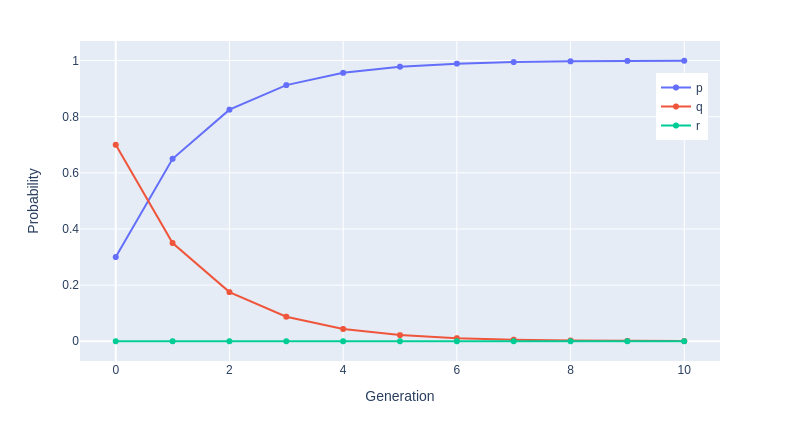
\includegraphics[width=\textwidth]{graph.png}
    \caption{Probability Dynamics}
    \label{fig:probability_dynamics}
\end{figure}
\subsection{Use of Linear Algebra}
In the given problem, we are interested in determining the long-term distribution of genotypes in a population. To analyze this, we formulate the problem using matrix notation and apply concepts from linear algebra. \\

1. \textbf{Transition Matrix:} The given Punnett square probabilities are represented using a transition matrix, denoted as $\mathbf{P}$. This matrix describes the probabilities of transitioning from one generation to the next.

2. \textbf{Matrix Equation:} We express the distribution of genotypes in each generation using a matrix equation, specifically $\mathbf{X}^{(n)} = \mathbf{P}\mathbf{X}^{(n-1)}$, where $\mathbf{X}^{(n)}$ represents the genotype proportions in the $n$th generation.

3. \textbf{Eigenvectors and Eigenvalues:} To analyze the long-term behavior of the system, we determine the eigenvalues and eigenvectors of the transition matrix $\mathbf{P}$. The eigenvalues represent the growth rates or proportions associated with each genotype in the long run, while the eigenvectors indicate the corresponding directions or patterns.

4. \textbf{Diagonalization:} By diagonalizing the transition matrix $\mathbf{P}$, we express it as a product of three matrices: $\mathbf{C}$, $\mathbf{D}$, and $\mathbf{C}^{-1}$. Here, $\mathbf{C}$ is the matrix consisting of eigenvectors, $\mathbf{D}$ is the diagonal matrix with eigenvalues, and $\mathbf{C}^{-1}$ is the inverse of $\mathbf{C}$.

5. \textbf{Long-Term Distribution:} Using the diagonalized form of $\mathbf{P}$, we can compute the long-term distribution of genotypes by applying the matrix equation $\mathbf{X}^{(n)} = \mathbf{C}\mathbf{D}^n\mathbf{C}^{-1}\mathbf{X}^{(0)}$, where $\mathbf{D}^n$ represents raising the diagonal matrix $\mathbf{D}$ to the power of $n$.

By leveraging these concepts from linear algebra, we analyzes the steady-state distribution of genotypes in the population, understand the long-term behavior, and make predictions based on the initial genotype proportions.
\section{Conclusion}
Linear algebra plays a crucial role in understanding and analyzing genetic phenomena. It provides powerful tools for studying the relationships between alleles, genotypes, and phenotypes in populations. As genetics advances, the integration of linear algebraic techniques will become even more significant, enabling us to extract insights from vast datasets, uncover genetic patterns, and make predictions about genes and populations. Linear algebra will continue to be essential for modeling and understanding the intricate relationships in genetics, driving discoveries and advancements in the field.
\newpage
\begin{thebibliography}{1}
\bibitem{Book 1} Linear Algebra: A Modern Introduction by Robert Rogers and David Poole, 2nd edition
\bibitem{Book 2} Linear Algebra. K. Hoffman, and R. Kunze. PHI Learning, Second edition, (2004 )
\bibitem{Book 3} Cubero, J. I. (2013). Introduction to plant breeding. Madrid: Mundi-Prensa Libros
\bibitem{Book 4} Gordillo, W., \& Pino-Fan, L. (2016). A proposed reconstruction of the holistic meaning of the antiderivative.. Bolema: Boletim de Educação Matemática, 30(55), 535-558. doi: 10.1590/1980-4415v30n55a12
\bibitem{Book 5} Zhang, Jiapu.\textit{Molecular Structures and Structural Dynamics of Prion Proteins and Prions}, Springer, 2015.
\bibitem{Paper 1} Grossman, S. I.,\& Flores,J .J (2012). Linear algebra, México: McGraw Hill Educación.
\bibitem{Paper 2} Jimenez, J. A. (2004). Class Notes Linear Algebra II With Applications in Statistics, Bogotá: Universidad Nacional de Colombia
\bibitem{Paper 3} Johnson, R., \& Onwuegbuzie, A. (2004). Mixed methods research: a research paradigm whose time has come. Educational Research, 33(7), 14-26
\bibitem{Paper 4} Pino-Fan, L., Font, V., Gordillo, W., Larios, V. \& Breda, A. (2018). Analysis of the meanings of the antiderivate used by students of the first engineering courses. International Journal of Science and Mathematics Education, 16(6), 1091-1113. doi:10.1007/s10763-017-9826-2
\bibitem{Paper 5} Sturtevant, A. H. (1965). A History of Genetics. California: Institute of Technology
\bibitem{Paper 6} Wolfram Research, Inc., Wolfram|Alpha Notebook Edition, Champaign, IL (2022).
\end{thebibliography}



\end{document}

